% Theory note: non-perturbative IP-UCC. Preamble copied from manuscript/manuscript.tex. Compile in a copy, never in manuscript/.
\documentclass[aip,jcp,reprint,noshowkeys,superscriptaddress]{revtex4-2}
\usepackage{graphicx,dcolumn,bm,xcolor,microtype,multirow,amscd,amsmath,amssymb,amsfonts,physics,wrapfig,bbold,siunitx,xspace,braket,txfonts}
\usepackage[version=4]{mhchem}

\usepackage[utf8]{inputenc}
\usepackage[T1]{fontenc}
\usepackage[english]{babel}
\babelprovide[import=en]{en} % bib entries carry language = {en}
\usepackage{feynmp-auto}
\usepackage{longtable}
\usepackage{rotating}
\usepackage{hyperref}
\usepackage[compat=1.0.0]{tikz-feynman}

\hypersetup{
    colorlinks,
    linkcolor={red!50!black},
    citecolor={red!70!black},
    urlcolor={red!80!black}
}

\usepackage{listings}
\definecolor{codegreen}{rgb}{0.58,0.4,0.2}
\definecolor{codegray}{rgb}{0.5,0.5,0.5}
\definecolor{codepurple}{rgb}{0.25,0.35,0.55}
\definecolor{codeblue}{rgb}{0.30,0.60,0.8}
\definecolor{backcolour}{rgb}{0.98,0.98,0.98}
\definecolor{mygray}{rgb}{0.5,0.5,0.5}

\definecolor{sqred}{rgb}{0.85,0.1,0.1}
\definecolor{sqgreen}{rgb}{0.25,0.65,0.15}
\definecolor{sqorange}{rgb}{0.90,0.50,0.15}
\definecolor{sqblue}{rgb}{0.10,0.3,0.60}

\lstdefinestyle{mystyle}{
    backgroundcolor=\color{backcolour},
    commentstyle=\color{codegreen},
    keywordstyle=\color{codeblue},
    numberstyle=\tiny\color{codegray},
    stringstyle=\color{codepurple},
    basicstyle=\ttfamily\footnotesize,
    breakatwhitespace=false,
    breaklines=true,
    captionpos=b,
    keepspaces=true,
    numbers=left,
    numbersep=5pt,
    numberstyle=\ttfamily\tiny\color{mygray},
    showspaces=false,
    showstringspaces=false,
    showtabs=false,
    tabsize=2
  }

  \newcolumntype{d}{D{.}{.}{-1}}

  \lstset{style=mystyle}

\newcommand{\cre}[1]{a_{#1}^\dagger}
\newcommand{\ani}[1]{a_{#1}} 

\newcommand{\fcre}[1]{\Hat{a}_{#1}^{\dag}}
\newcommand{\fani}[1]{\Hat{a}_{#1}}

\newcommand{\bfcre}[1]{\Hat{\Bar{a}}_{#1}^{\dag}}
\newcommand{\bfani}[1]{\Hat{\Bar{a}}_{#1}}

\newcommand{\bcre}[1]{\Hat{b}_{#1}^{\dag}}
\newcommand{\bani}[1]{\Hat{b}_{#1}}

\newcommand{\bacre}[1]{\Bar{b}_{#1}^{\dag}}
\newcommand{\baani}[1]{\Bar{b}_{#1}}

\newcommand{\bbacre}[1]{\dBar{b}_{#1}^{\dag}}
\newcommand{\bbaani}[1]{\dBar{b}_{#1}}

\newcommand{\bbcre}[1]{\Hat{\beta}_{#1}^{\dag}}
\newcommand{\bbani}[1]{\Hat{\beta}_{#1}}


\newcommand{\ccre}[1]{\Hat{c}_{#1}^{\dag}}
\newcommand{\cani}[1]{\Hat{c}_{#1}}

\newcommand{\bccre}[1]{\Hat{\Bar{c}}_{#1}^{\dag}}
\newcommand{\bcani}[1]{\Hat{\Bar{c}}_{#1}}


\newcommand{\dcre}[1]{\Hat{d}_{#1}^{\dag}}
\newcommand{\dani}[1]{\Hat{d}_{#1}}

\newcommand{\bdcre}[1]{\Hat{\Bar{d}}_{#1}^{\dag}}
\newcommand{\bdani}[1]{\Hat{\Bar{d}}_{#1}}

\usepackage{accents}
\newcommand{\dBar}[1]{\Bar{\Bar{#1}}}

\newcommand{\NO}[1]{\{#1\}} 
\newcommand{\ERI}[2]{\braket{#1|#2}}
\newcommand{\sERI}[2]{(#1|#2)}
\newcommand{\dbERI}[2]{\mel{#1}{}{#2}}
\newcommand{\e}[2]{\epsilon_{#1}^{#2}}
\newcommand{\eHF}[1]{\epsilon_{#1}^\text{HF}}
\newcommand{\eKS}[1]{\epsilon_{#1}^\text{KS}}
\newcommand{\Om}{\Omega}
\newcommand{\om}{\omega}

\newcommand{\rev}[1]{\textcolor{black}{#1}}
\newcommand{\revtwo}[1]{\textcolor{black}{#1}}

\newcommand{\titou}[1]{\textcolor{red}{#1}}
\newcommand{\petros}[1]{\textcolor{cyan}{#1}}
\newcommand{\jt}[1]{\textcolor{orange}{#1}}
\newcommand{\ag}[1]{\textcolor{teal}{#1}}
\newcommand{\ai}[1]{\textcolor{magenta}{#1}}
\newcommand{\trashPFL}[1]{\textcolor{red}{\sout{#1}}}
\newcommand{\trashMPK}[1]{\textcolor{cyan}{\sout{#1}}}
\newcommand{\PFL}[1]{\titou{(\underline{\bf PFL}: #1)}}
\newcommand{\MPK}[1]{\petros{(\underline{\bf MPK}: #1)}}
\newcommand{\JT}[1]{\jt{(\underline{\bf JT}: #1)}}
\newcommand{\AG}[1]{\ag{(\underline{\bf AG}: #1)}}
\newcommand{\AI}[1]{\ai{(\underline{\bf AI}: #1)}}
\newcommand{\eqrref}[1]{Eq.~\eqref{#1}}
\newcommand{\fnm}{\footnotemark}
\newcommand{\fnt}{\footnotetext}

\newcommand{\GOWO}{\text{$G_0W_0$}}
\newcommand{\drCCD}{\text{drCCD}}
\newcommand{\IP}{\text{IP}}
\newcommand{\EA}{\text{EA}}
\newcommand{\IPEA}{\text{IP/EA}}
\newcommand{\EOM}{\text{EOM}}

\newcommand{\TCC}{\text{TCC}}
\newcommand{\ECC}{\text{ECC}}

\newcommand{\ba}{\boldsymbol{a}}
\newcommand{\bb}{\boldsymbol{b}}
\newcommand{\bbb}{\boldsymbol{\beta}}
\newcommand{\bc}{\boldsymbol{c}}
\newcommand{\bbc}{\Bar{\bc}}
\newcommand{\bd}{\boldsymbol{d}}
\newcommand{\bbd}{\Bar{\bd}}
\newcommand{\bx}{\boldsymbol{x}}
\newcommand{\bA}{\boldsymbol{A}}
\newcommand{\bB}{\boldsymbol{B}}
\newcommand{\bC}{\boldsymbol{C}}
\newcommand{\bD}{\boldsymbol{D}}
\newcommand{\bG}{\boldsymbol{G}}
\newcommand{\bX}{\boldsymbol{X}}
\newcommand{\bY}{\boldsymbol{Y}}
\newcommand{\bT}{\boldsymbol{T}}
\newcommand{\bt}{\boldsymbol{t}}
\newcommand{\bR}{\boldsymbol{R}}
\newcommand{\br}{\boldsymbol{r}}
\newcommand{\bE}{\boldsymbol{E}}
\newcommand{\bM}{\boldsymbol{M}}
\newcommand{\bN}{\boldsymbol{N}}
\newcommand{\bH}{\boldsymbol{H}}
\newcommand{\bO}{\boldsymbol{0}}
\newcommand{\bI}{\boldsymbol{1}}
\newcommand{\bS}{\boldsymbol{S}}
\newcommand{\bz}{\boldsymbol{z}}
\newcommand{\bV}{\boldsymbol{V}}
\newcommand{\bff}{\boldsymbol{f}}
\newcommand{\bLam}{\boldsymbol{\Lambda}}
\newcommand{\blam}{\boldsymbol{\lambda}}
\newcommand{\bgam}{\boldsymbol{\gamma}}
\newcommand{\bOm}{\boldsymbol{\Omega}}
\newcommand{\bSig}{\boldsymbol{\Sigma}}
\newcommand{\beps}{\boldsymbol{\epsilon}}

\newcommand{\hT}{\Hat{T}}
\newcommand{\hW}{\Hat{W}}
\newcommand{\hF}{\Hat{F}}
\newcommand{\hL}{\Hat{L}}
\newcommand{\hR}{\Hat{R}}
\newcommand{\hH}{\Hat{H}}
\newcommand{\hbH}{\Bar{H}}
\newcommand{\hbbH}{\dBar{H}}
\newcommand{\hI}{\Hat{1}}
\newcommand{\hV}{\Hat{V}}
\newcommand{\hZ}{\Hat{Z}}
\newcommand{\hLam}{\Hat{\Lambda}}
\newcommand{\htau}{\Hat{\tau}}
\newcommand{\hXi}{\Hat{\Xi}}

\newcommand{\cL}{\mathcal{L}}
\newcommand{\wtH}{\widetilde{H}}
\newcommand{\wtV}{\widetilde{V}}

\newcommand{\T}[1]{#1^{\intercal}}
\newcommand{\Ec}{E_\text{c}}

%%% Text acronyms and abbreviations %%%

\newcommand{\FCI}{\text{FCI}}
\newcommand{\HF}{\text{HF}}
\newcommand{\MCSCF}{\text{MCSCF}}
\newcommand{\occ}{\text{occ}}
\newcommand{\vir}{\text{vir}}
\newcommand{\HOMO}{\text{HOMO}}
\newcommand{\LUMO}{\text{LUMO}}
\newcommand{\nuc}{\text{nuc}}
\newcommand{\KS}{\text{KS}}
\newcommand{\RPA}{\text{RPA}}
\newcommand{\phRPA}{\text{ph-RPA}}
\newcommand{\ppRPA}{\text{pp-RPA}}
\newcommand{\h}{\text{1h}}
\newcommand{\p}{\text{1p}}
\newcommand{\hp}{\text{1h+1p}}
\newcommand{\hhp}{\text{2h1p}}
\newcommand{\pph}{\text{2p1h}}
\newcommand{\ph}{\text{ph}}
\newcommand{\eh}{\text{eh}}
\newcommand{\he}{\text{he}}
\newcommand{\ee}{\text{ee}}
\newcommand{\teh}{\overline{\text{eh}}}
\newcommand{\pp}{\text{pp}}
\newcommand{\hh}{\text{hh}}
\newcommand{\dRPA}{\text{dRPA}}
\newcommand{\TDA}{\text{TDA}}
\newcommand{\RPAx}{\text{RPAx}}
\newcommand{\QP}{\textsc{quantum package}}
\newcommand{\Hxc}{\text{Hxc}}
\newcommand{\xc}{\text{xc}}
\newcommand{\x}{\text{x}}

\newcommand{\ldr}{\text{$\lambda$-dr}}
\newcommand{\dr}{\text{dr}}
\newcommand{\ii}{\text{i}}
\newcommand{\SupInf}{\textcolor{blue}{Supporting Information}\xspace}

\newcommand{\stkout}[1]{\ifmmode\text{\sout{\ensuremath{#1}}}\else\sout{#1}\fi}

% addresses
\newcommand{\UnHam}{Department of Chemistry, University of Hamburg, 22761 Hamburg, Germany; The Hamburg Centre for Ultrafast Imaging (CUI), Hamburg 22761, Germany}
\newcommand{\LCPQ}{Univ Toulouse, CNRS, Laboratoire de Chimie et Physique Quantiques, Toulouse, France}

\newcommand{\VUA}{Department of Chemistry and Pharmaceutical Sciences, Vrije Universiteit, De Boelelaan 1105, 1081 HV Amsterdam, The Netherlands}




\newcommand{\Hb}{\hat{\bar{H}}}
\newcommand{\hs}{\hat{\sigma}}
\newcommand{\hts}{\hat{\tilde{\sigma}}}
\newcommand{\Ord}{\mathcal{O}}

\begin{document}

\title{Ionization potentials from a non-perturbative unitary coupled-cluster ground state}

\author{Arno Förster}
	\affiliation{\VUA}

\begin{abstract}
We derive an ionization method that keeps the Hermitian, frequency-independent eigenvalue problem of non-Dyson ADC but replaces its perturbatively expanded ground state by a unitary coupled-cluster (UCC) ground state solved at the physical interaction strength.
The method has three truncations: the excitation rank $r$ of the cluster operator, the highest cation excitation class $K$, and the number $M$ of nested commutators.
The construction is the self-consistent electron propagator of Prasad, Pal, and Mukherjee; its only practical realization so far, IP-qUCCSD of Zhang and Liu, stops at singles and doubles in the ground state and at the 2h1p configurations in the cation.
We show that the ionization potential is exact through an order set by the smallest of three limits, one for each truncation, and that an odd number of commutators never gains an order over the next lower even number.
\end{abstract}

\maketitle

\section{Setting}

We argue that a good approximation to the IP part of $\bG$ should therefore have a ground state that is not treated by perturbation theory, be complete order by order, and lead to a Hermitian, frequency-independent eigenvalue problem.
ADC($n$) and its UCC analogue IP-UCC($n$)\cite{Mertins_1996,Hodecker_2022} have the second and third property.
IP-EOM-CC\cite{Stanton_1993a} has the first and second, but its eigenvalue problem is not Hermitian.

A non-perturbatve gound state is arguably of utmost importance. For Ne in an augmented basis, the Møller--Plesset (MP) series of the ground state diverges because of a back-door intruder inside the unit circle.\cite{Olsen1996,Olsen_2000}
GF($n$) and ADC($n$) inherit this divergence, since both contain the MP series of the ground state through order $n$.
IP-EOM-CC does not, because it solves the ground state at the physical coupling.

We here detail derivations an analysis of a self-energy construction based on the UCC ansatz that 
fulfills all three properties, following the ideas of \citet{Liu_2018}, \citet{Liu_2021} and \citet{Zhang_2026}.

The setting is as follows: we scale the interaction as
\begin{equation}
\hH(\lambda) = \hF + \lambda (\hH - \hF),
\label{eq:Hlambda}
\end{equation}
with $\hF$ the canonical Hartree--Fock (HF) Fock operator, so that the physical system is reached at unit coupling.
We follow one occupied orbital $k$ and the cation state $\ket{\Psi_k}$ connected to the Koopmans determinant.
Its ionization potential (IP) is
\begin{equation}
\IP_k(\lambda) = E_{N-1,k}(\lambda) - E_0(\lambda).
\label{eq:IP}
\end{equation}
A method is exact through order $n$ if its IP agrees with Eq.~\eqref{eq:IP} through $\lambda^n$.


\section{Ground state}

We write the ground state as
\begin{equation}
\ket{\Psi_0} = e^{\hs}\ket{\Phi_0}, \qquad \hs = \hT - \hT^\dagger,
\label{eq:ucc}
\end{equation}
where $\hT$ contains all excitation operators up to rank $r$ with real amplitudes.\cite{Kutzelnigg_1982,Bartlett_1989,Taube_2006}
Rank two gives UCCSD, rank three UCCSDT, and rank four UCCSDTQ.
Because $\hs$ is anti-Hermitian, $e^{\hs}$ is unitary, and the transformed Hamiltonian
\begin{equation}
\Hb = e^{-\hs} \hH e^{\hs}
\label{eq:Hbar}
\end{equation}
is Hermitian.
We fix the amplitudes at the physical coupling, either by the projective conditions
\begin{equation}
\braket{\Phi_\nu | \Hb | \Phi_0} = 0
\label{eq:proj}
\end{equation}
or by the generalized Brillouin conditions
\begin{equation}
\braket{\Psi_0 | [\hH, \hat\tau_\nu - \hat\tau_\nu^\dagger] | \Psi_0} = 0,
\label{eq:gbt}
\end{equation}
for every excitation $\hat\tau_\nu$ up to rank $r$.
In both cases the ground-state energy is
\begin{equation}
E_0 = \braket{\Phi_0 | \Hb | \Phi_0} = \braket{\Psi_0 | \hH | \Psi_0}.
\label{eq:E0}
\end{equation}
If all ranks are kept, both sets of conditions make $\ket{\Psi_0}$ an exact eigenstate,
\begin{equation}
\Hb\ket{\Phi_0} = E_0\ket{\Phi_0}.
\label{eq:exact}
\end{equation}
With truncated rank, the two sets of conditions give different amplitudes.

In practice, $\Hb$ is evaluated by the commutator expansion, truncated after $M$ nested commutators,
\begin{equation}
\Hb_M = \sum_{m=0}^{M} \frac{1}{m!}\, [\dots[\hH, \underbrace{\hs], \dots, \hs]}_{m}.
\label{eq:bch}
\end{equation}
Every term is Hermitian, so $\Hb_M$ is Hermitian for every $M$.
The exact exponential is the limit of infinitely many commutators.

\section{Ionized states}

The intermediate states are
\begin{equation}
\ket{\tilde\Psi_J} = e^{\hs} \ket{\Phi_J},
\label{eq:is}
\end{equation}
with $\ket{\Phi_J}$ the cation determinants of the classes up to $K$.
A determinant of class $c$ has $c+1$ holes and $c$ particles. The first three classes are the 1h, 2h1p, and 3h2p determinants,
\begin{equation}
\hat{a}_i\ket{\Phi_0}, \quad \hat{a}_a^\dagger \hat{a}_j \hat{a}_i \ket{\Phi_0}, \quad \hat{a}_a^\dagger \hat{a}_b^\dagger \hat{a}_k \hat{a}_j \hat{a}_i \ket{\Phi_0},
\label{eq:classes}
\end{equation}
with $i,j,k$ occupied and $a,b$ virtual orbitals.
The first level keeps 1h and 2h1p, like ADC(2), ADC(3), and IP-EOM-CCSD; the second adds 3h2p, like ADC(4), ADC(5), and IP-EOM-CCSDT; the third adds 4h3p.
Table~\ref{tab:levels} lists the combinations of ground state and cation space for UCCSD, UCCSDT, and UCCSDTQ.
The operator $\hs$ is the same as in the ground state, applied in the cation space.
Since $e^{\hs}$ is unitary, the intermediate states are orthonormal without a Gram--Schmidt step.
The IPs are the eigenvalues of
\begin{equation}
\mathcal{M}_{IJ} = \braket{\Phi_I | \Hb_M - E_0 | \Phi_J},
\label{eq:M}
\end{equation}
and the IP of orbital $k$ is the eigenvalue with the largest weight on the Koopmans determinant.
$\mathcal{M}$ is real symmetric and independent of the frequency.
With all classes and the exact exponential, its eigenvalues are exact for any $\hs$.
With fewer classes, they are Ritz values of the exact Hamiltonian in the space of Eq.~\eqref{eq:is}.

\citet{Mertins_1996} showed that ADC and IP-UCC follow from the same intermediate-state framework.
They differ in the intermediate states: ADC orthonormalizes the states obtained by applying the cation operators to the correlated ground state, while UCC uses Eq.~\eqref{eq:is}.\cite{Mertins_1996,Schirmer_1991}
If $\hs$ is expanded in $\lambda$ and $\mathcal{M}$ is truncated by the ADC rule, one obtains the perturbative IP-UCC($n$).\cite{Mertins_1996,Hodecker_2022}
IP-UCC($n$) equals ADC($n$) through third order and differs from fourth order on.\cite{Liu_2018,Hodecker_2022}
For Ne in aug-cc-pVDZ, the two stay within a few meV of each other and diverge alike.
The present method differs from IP-UCC($n$) only in the ground state, which is solved at the physical coupling and not expanded.

Key to the construction here is that the UCC ansatz is used to solve for the ground state non-perturbatively.
The construction itself has first been presented by \citet{prasad1985some} 
but practical realizations are more recent.
\citet{Liu_2018} truncated both the amplitude equations and the blocks of the secular matrix by perturbation order (UCC3) but solved the amplitudes iteratively.
\citet{Liu_2021} truncated by the number of commutators instead (qUCCSD): double commutators in the amplitude equations, triple commutators in the energy, and one commutator less in each block of the secular matrix as one moves away from the singles.
\citet{Zhang_2026} carried this over to IPs and electron affinities.
Their IP-qUCCSD keeps the 1h and 2h1p configurations, with double commutators in the 1h block, single commutators in the coupling block, and the bare Hamiltonian in the 2h1p block; it is correct through third order and contains no triples.
\citet{Asthana_2023} evaluated the same eigenvalue problem with a near-exact ground state on a quantum computer, with 1h and 2h1p operators and minimal basis sets.
Non of these works contain cation classes beyond 2p1h.
We show here that these are crucial for useful accuracy of this method that matches its rather high scaling.

\section{Order consistency}

We assume that orbital $k$ is non-degenerate within its symmetry block, and that no other cation determinant of that block has the same zeroth-order energy as the Koopmans determinant.
The IP is then an isolated, simple eigenvalue for small $\lambda$, and all quantities below are analytic in $\lambda$.

\subsection{Exact amplitudes}

We expand the exact cluster operator as
\begin{equation}
\hs(\lambda) = \sum_{s\geq1} \lambda^s \hs_s.
\label{eq:sigmaexp}
\end{equation}
At order $s$, Eq.~\eqref{eq:proj} or \eqref{eq:gbt} reads
\begin{equation}
\Delta_\nu\, t_{s,\nu} = R_{s,\nu}[\hs_1,\dots,\hs_{s-1}] \;.
\label{eq:order_s}
\end{equation}
$\Delta_\nu$ is the positive orbital-energy difference of excitation $\nu$ and a right-hand side that depends only on lower orders.
At first order, this gives the MP1 doubles,
\begin{equation}
[\hF, \hs_1] = -\hV_\mathrm{od},
\label{eq:sigma1}
\end{equation}
where $\hV_\mathrm{od}$ is the double-excitation and double-de-excitation part of $\hH - \hF$ in normal order with respect to $\ket{\Phi_0}$.
By virtue of the linked-diagram structure of the cluster operator, $\hs_s$ is connected and has excitation rank
\begin{equation}
\mathrm{rank}(\hs_s) \le s + 1.
\label{eq:rank}
\end{equation}

\subsection{Order relations}

A nested commutator of $\hH - \hF$ with $\hs_{s_1},\dots,\hs_{s_m}$ is of order $s$, the sum of the $s_i$ plus one.
Each commutator contracts at least one index, so with Eq.~\eqref{eq:rank} the term is at most an $(s+1)$-body operator.
The same bound holds for the commutators of $\hF$.
Such an operator changes the number of virtual electrons by at most $s+1$, and by exactly $s+1$ only if it is a pure excitation or de-excitation.
By Eq.~\eqref{eq:exact}, the pure excitation part of $\Hb$ vanishes at every order, and by Hermiticity so does the pure de-excitation part.
The order-$s$ part of the block between classes $c$ and $l$ therefore satisfies
\begin{equation}
\Hb^{(s)}_{cl} = 0 \qquad \text{for } s < |c-l|.
\label{eq:orderrel}
\end{equation}
These are the canonical order relations of the ISR,\cite{Mertins_1996,Schirmer_2018} here for the UCC intermediate states.
Each step between classes costs at least as many powers of $\lambda$ as the classes are apart.
The exact cation eigenvector in the transformed basis,
\begin{equation}
\ket{X} = e^{-\hs}\ket{\Psi_k},
\label{eq:X}
\end{equation}
normalized to unit weight on the Koopmans determinant, therefore has class components
\begin{equation}
X_c = \Ord(\lambda^c).
\label{eq:Xc}
\end{equation}

\subsection{Ground-state rank}

Let $\hts$ be the solution of Eq.~\eqref{eq:proj} or \eqref{eq:gbt} with ranks up to $r$.
Below order $r$, the exact amplitudes have rank at most $r$ by Eq.~\eqref{eq:rank}, so the truncation removes nothing and Eq.~\eqref{eq:order_s} is the same equation in both cases.
By induction,
\begin{equation}
\hts - \hs = \Ord(\lambda^r).
\label{eq:sigmaerr}
\end{equation}
The difference of the two normalized ground states,
\begin{equation}
\ket{\delta} = e^{\hts}\ket{\Phi_0} - e^{\hs}\ket{\Phi_0} = \Ord(\lambda^r),
\label{eq:delta}
\end{equation}
enters the energy of Eq.~\eqref{eq:E0} quadratically,
\begin{equation}
\tilde E_0 - E_0 = \braket{\delta | \hH - E_0 | \delta} = \Ord(\lambda^{2r}).
\label{eq:E0err}
\end{equation}
This holds for both sets of conditions, because with the exact exponential the energy is the expectation value of a normalized state.
UCCSD is thus exact through third order, UCCSDT through fifth, and UCCSDTQ through seventh.
It shares this property with EOM-IP-CCSD/CCSDT/CCSDTQ.

\subsection{Cation classes}

Let $\hat{P}$ project onto the kept classes and $\hat{Q}$ onto the rest.
In the basis of the truncated amplitudes, the exact cation eigenvector is
\begin{equation}
\ket{Y} = e^{-\hts}e^{\hs}\ket{X}.
\label{eq:Y}
\end{equation}
By Eq.~\eqref{eq:sigmaerr}, the operator in front of $\ket{X}$ differs from the identity at order $r$, and with Eq.~\eqref{eq:Xc}
\begin{equation}
\hat{Q}\ket{Y} = \Ord(\lambda^{\min(K+1,\,r)}).
\label{eq:QY}
\end{equation}
With the exact exponential, the eigenvalue $\theta$ of $\hat{P}\Hb\hat{P}$ is a Ritz value, and its error is quadratic in the part of the exact eigenvector outside the space,
\begin{equation}
\theta - E_{N-1,k} = \Ord(\|\hat{Q}\ket{Y}\|^2).
\label{eq:ritz}
\end{equation}
This follows because $\hat{P}\ket{Y}$ is an approximate eigenvector of $\hat{P}\Hb\hat{P}$ with a residual proportional to $\hat{Q}\ket{Y}$, and the eigenvalue error of an isolated eigenvalue of a Hermitian matrix is quadratic in the residual.
Together with Eq.~\eqref{eq:E0err}, the IP error is
\begin{equation}
\IP_k^{\,r,K} - \IP_k = \Ord(\lambda^{2\min(K+1,\,r)}).
\label{eq:rKerr}
\end{equation}
The ground-state rank limits the order through the ground-state energy and through the intermediate states; the cation classes limit it through the size of the space.
The matched choice keeps one class fewer than the rank, and its class requirement is the same as for ADC($n$).
For the polarization propagator with singles and doubles, \citet{Liu_2018} gave the special case of this argument: because $\Hb$ is Hermitian and its double excitations vanish, the triples reach singly excited states only at fourth order, whereas in EOM-CC they enter at third order.

\subsection{Commutator truncation}

With finitely many commutators, the omitted part of $\Hb$ is
\begin{equation}
\Hb - \Hb_M = \sum_{m > M} \frac{1}{m!}\, [\dots[\hH, \underbrace{\hs], \dots, \hs]}_{m}.
\label{eq:rest}
\end{equation}
Every $\hs_s$ is at least of first order, so the lowest-order term has $M+1$ factors $\hs_1$ acting on $\hF$.
With Eq.~\eqref{eq:sigma1}, it is
\begin{equation}
\left(\Hb - \Hb_M\right)^{(M+1)} = -\frac{1}{(M+1)!}\, [\dots[\hV_\mathrm{od}, \underbrace{\hs_1], \dots, \hs_1]}_{M}.
\label{eq:leading}
\end{equation}
This is a product of $M+1$ operators, each of which changes the number of virtual electrons by two in either direction.
Its matrix elements between classes $c$ and $l$ therefore vanish unless
\begin{equation}
c - l \equiv 2(M+1) \pmod 4.
\label{eq:parity}
\end{equation}
For odd $M$, Eq.~\eqref{eq:leading} has diagonal elements.
It changes the ground-state energy and the Koopmans diagonal element at order $M+1$, and the two changes do not cancel in general.
For even $M$, Eq.~\eqref{eq:leading} vanishes in every diagonal block, including the ground-state energy, and couples only classes at least two apart.
An error in such a block enters the IP at least two orders later.
Eq.~\eqref{eq:leading} also changes the doubles amplitudes at order $M+1$.
Through its commutator with $\hF$, this change again couples only classes two apart, and it changes the ground-state energy only at higher order.
The first error in the IP is then of order $M+2$.
\citet{Liu_2021} observed the same imbalance from the size of the terms: the commutator of $\hF$ with $\hs$ is as large as the fluctuation potential, so in the plain commutator series the commutators of $\hF$ must be kept to one more order than those of the fluctuation potential.
They avoid this by a Bernoulli-number expansion of $\Hb$ in which $\hF$ enters only through a single commutator.\cite{Liu_2018,Liu_2021}
Our count of commutators refers to the plain series, Eq.~\eqref{eq:bch}.

Together with Eq.~\eqref{eq:rKerr}, the IP is exact through order
\begin{equation}
n = \min\left(2K+1,\; 2r-1,\; 2\lfloor M/2\rfloor + 1\right).
\label{eq:rule}
\end{equation}
The matched hierarchy keeps one class fewer than the rank and twice that number of commutators: UCCSD with double commutators is exact through third order, UCCSDT with four commutators through fifth, and UCCSDTQ with six through seventh.

\section{Working equations for UCCSD with 3h2p}

We now write out the matrix of Eq.~\eqref{eq:M} for a UCCSD ground state and the 1h, 2h1p, and 3h2p configurations.
The cation basis is
\begin{align}
\ket{\Phi_i} &= \hat{a}_i\ket{\Phi_0}, \qquad
\ket{\Phi_{ij}^{a}} = \hat{a}_a^\dagger \hat{a}_j \hat{a}_i\ket{\Phi_0}, \nonumber\\
\ket{\Phi_{ijk}^{ab}} &= \hat{a}_a^\dagger \hat{a}_b^\dagger \hat{a}_k \hat{a}_j \hat{a}_i\ket{\Phi_0},
\label{eq:basis}
\end{align}
with ordered index pairs and triples, and the cluster operator is
\begin{equation}
\hs = \sum_{ia} t_i^a \big(\hat{a}_a^\dagger \hat{a}_i - \hat{a}_i^\dagger \hat{a}_a\big)
+ \frac{1}{4}\sum_{ijab} t_{ij}^{ab} \big(\hat{a}_a^\dagger \hat{a}_b^\dagger \hat{a}_j \hat{a}_i - \hat{a}_i^\dagger \hat{a}_j^\dagger \hat{a}_b \hat{a}_a\big)
\label{eq:sigmaSD}
\end{equation}
with real amplitudes.
The doubles amplitudes are of first order and the singles of second order.
The matrix is symmetric, so the blocks below the diagonal follow by transposition.

Each block is given through the order that a third-order IP needs, and the 3h2p blocks at their leading order.
These are the terms of the Bernoulli-form transformed Hamiltonian of \citet{Liu_2018} up to the double commutator, selected by their leading order.
The 1h block uses the occupied-occupied part of the UCC3 Hamiltonian of \citet{Liu_2018}, and the 1h/2h1p block its two-body part with three occupied indices.
Elements that contain the residual of the amplitude equations are dropped, because the residual vanishes for converged amplitudes.
We denote by $\mathcal{S}_{ij}$ the sum of a term and the same term with $i$ and $j$ exchanged, by $P(ij)$ the corresponding difference, and by $P(i/jk)$ the term minus the terms with $i$ exchanged with $j$ and with $k$.

The 1h block through third order is
\begin{align}
\mathcal{M}_{ij} ={}& -\epsilon_i\delta_{ij}
- \mathcal{S}_{ij}\Big[\sum_{ka}\braket{ik||ja}t_k^a + \frac{1}{4}\sum_{kab}\braket{ik||ab}t_{jk}^{ab} \nonumber\\
&+ \frac{1}{2}\sum_{klabc}\braket{ic||al}t_{jk}^{ab}t_{kl}^{bc} + \frac{1}{8}\sum_{klmab}\braket{im||kl}t_{jm}^{ab}t_{kl}^{ab}\Big] \nonumber\\
&+ \frac{1}{2}\sum_{klmab}\braket{im||jl}t_{kl}^{ab}t_{km}^{ab} - \frac{1}{2}\sum_{klabc}\braket{ic||jb}t_{kl}^{ab}t_{kl}^{ac}.
\label{eq:M11}
\end{align}
The first-order part vanishes for HF orbitals.
With first-order amplitudes, the second-order part is a product of bare integrals,
\begin{equation}
\mathcal{M}^{(2)}_{ij} = \frac{1}{4}\sum_{kab}\left[\frac{\braket{ik||ab}\braket{ab||jk}}{\epsilon_a+\epsilon_b-\epsilon_j-\epsilon_k} + \frac{\braket{jk||ab}\braket{ab||ik}}{\epsilon_a+\epsilon_b-\epsilon_i-\epsilon_k}\right].
\label{eq:M11two}
\end{equation}
This is the 2p1h branch of the second-order self-energy evaluated at the orbital energies and symmetrized, i.e., the pair correlation of the removed electron that the IP loses.
Non-Dyson ADC(2) contains the same term in its 1h block, where the affinity branch is folded statically into the ionization sector; its couplings to 2h1p are bare integrals.
The third-order part of Eq.~\eqref{eq:M11} contains the singles and the products of two doubles amplitudes.

The coupling of 1h to 2h1p through second order is
\begin{align}
\mathcal{M}_{i,jk}^{\;a} ={}& -\braket{jk||ia} - P(jk)\sum_{lb}\braket{jb||il}t_{kl}^{ab} \nonumber\\
&- \frac{1}{2}\sum_{bc}\braket{bc||ia}t_{jk}^{bc}.
\label{eq:M12}
\end{align}
The first term is the coupling of ADC(2); the other two are its second-order corrections, as in ADC(3).

The 2h1p block through first order is
\begin{align}
\mathcal{M}_{ij,kl}^{\,a,b} ={}& \delta_{ik}\delta_{jl}\delta_{ab}(\epsilon_a - \epsilon_i - \epsilon_j) + \delta_{ab}\braket{kl||ij} \nonumber\\
&- P(ij)P(kl)\,\delta_{ik}\braket{al||bj},
\label{eq:M22}
\end{align}
which is the 2h1p block of ADC(3).

The coupling of 1h to 3h2p starts at second order,
\begin{equation}
\mathcal{M}_{i,jkl}^{\;ab} = -P(l/jk)P(ab)\sum_{c}\braket{lc||ib}t_{jk}^{ac} - P(j/kl)\sum_{m}\braket{kl||im}t_{jm}^{ab}.
\label{eq:M13}
\end{equation}
There is no first-order coupling, in agreement with Eq.~\eqref{eq:orderrel}: the first-order part of the Hamiltonian that connects these classes is a pure double de-excitation, which the amplitude equations remove.
This coupling is the only place where the ground-state amplitudes enter the 3h2p configurations at this level.

The coupling of 2h1p to 3h2p is of first order,
\begin{align}
\mathcal{M}_{ij,klm}^{\,a,bc} ={}& -P(m/kl)\big[(\delta_{ik}\delta_{jl} - \delta_{il}\delta_{jk})\braket{ma||bc}\big] \nonumber\\
&- P(k/lm)P(ij)P(bc)\big[\delta_{ik}\delta_{ab}\braket{lm||jc}\big],
\label{eq:M23}
\end{align}
and the 3h2p block is diagonal at zeroth order,
\begin{equation}
\mathcal{M}_{ijk,lmn}^{\,ab,cd} = \delta_{il}\delta_{jm}\delta_{kn}\delta_{ac}\delta_{bd}(\epsilon_a + \epsilon_b - \epsilon_i - \epsilon_j - \epsilon_k).
\label{eq:M33}
\end{equation}
Both are blocks of the bare Hamiltonian, the same as in ADC(4).
With these blocks, the 3h2p configurations change the IP only from fourth order on, consistent with Eq.~\eqref{eq:rule} for UCCSD.
At the physical coupling they change it substantially (Table~\ref{tab:ne}).
These blocks illustrate the structure at the third-order level. The implementation keeps every term of the two-commutator transformed Hamiltonian in every block; Appendix~\ref{app:complete} gives the operator expressions from which the implementation is generated.

At this level, the method is the UCC counterpart of CC3.\cite{Christiansen_1995b,Koch_1997}
The 3h2p configurations enter as the triples do in CC3: with a diagonal block of orbital-energy differences, a first-order coupling to the configuration class below, and a coupling to the 1h states through the ground-state doubles amplitudes.
The two methods therefore share the cation configuration space and the scaling.
The ground state costs $N^6$ per iteration, and the most expensive steps of one cation product are the couplings of 1h to 3h2p in Eq.~\eqref{eq:M13}, with operation counts that scale as $o^4v^3 + o^5v^2$, i.e., as $N^7$.
The 2h1p/3h2p coupling of Eq.~\eqref{eq:M23} costs $o^3v^3 + o^4v^2$, and the 3h2p block only $o^3v^2$.
CCR and UCCSD differ in what the triples do. In CC3, the triples are needed for excitation energies correct through third order, because the non-Hermitian transformed Hamiltonian couples triples and singles at first order in one direction and at second order in the other.\cite{Liu_2018}
Here, the 3h2p configurations first change the IP at fourth order, and they act only through the resummation at the physical coupling, which Table~\ref{tab:ne} shows to be large.
CC3 also contains approximate triples in the ground state, which the UCCSD ground state does not.

\section{Comparison to Faddeev-ADC}

The working equations are also close to those of Faddeev-ADC, which couples the 2h1p configurations to the particle-particle and particle-hole pair channels.\cite{Barbieri_2001,Barbieri_2007}
With MP amplitudes, the UCC blocks reduce to those of ADC(3);\cite{Liu_2018} with cluster amplitudes, they keep the ADC form.
In the Galerkin form of the Faddeev pencil, the 2h1p configurations are dressed by the backward pair amplitudes.
Its Hamiltonian then contains the bare block, couplings linear in the amplitudes, and a term quadratic in them, and its metric is the identity minus the square of the amplitudes.
The two-commutator 2h1p block of UCC contains the same three kinds of terms: the single commutator gives the linear couplings, and the double commutator the quadratic terms, including the normalization pieces.
Because $e^{\hs}$ is unitary, the UCC intermediate states are orthonormal, and the content of the metric moves into the transformed Hamiltonian.
The explicit 3h2p configurations correspond to the five-line states that Faddeev-ADC(3) folds into its pair amplitudes.
The two constructions differ in three respects.
First, a pencil with a metric has the same eigenvalues as its symmetrically orthonormalized form, but the unitary rotation is a different orthonormalization, so the two agree only through third order, through which both contain ADC(3).
Second, the Faddeev metric comes from the negative norm of the backward components of each pair channel, as in the random-phase approximation, and need not stay positive at strong coupling, whereas the UCC states are normalized by construction.
Third, Faddeev-ADC solves each pair channel as a two-body problem with a spectator, or ties the channels together through common CCD amplitudes, whereas UCC has one set of amplitudes from the ground-state equations and no channel structure.
IP-UCC is therefore closest to Faddeev-ADC with common amplitudes, with UCC instead of CCD amplitudes and the metric absorbed by a unitary transformation.

\section{Formal scaling}

With the exact exponential, the cost is that of full configuration interaction; we use it only for the oracle tests.
With finitely many commutators, every term of Eq.~\eqref{eq:bch} is a connected product of the Hamiltonian and at most $M$ amplitude tensors, and the cost is polynomial.
The terms with one amplitude tensor cost as much as the coupled-cluster method of the same rank, and one product of $\mathcal{M}$ with a cation vector costs at least as much as IP-EOM-CC with the same classes,
\begin{equation}
\text{ground state} \sim N^{2r+2}, \qquad \text{cation} \sim N^{2K+3}.
\label{eq:scaling}
\end{equation}
For UCCSD, the ground state thus costs at least $N^6$ per iteration, for UCCSDT $N^8$, and for UCCSDTQ $N^{10}$, as in CCSD, CCSDT, and CCSDTQ.
One cation product costs at least $N^5$ with 2h1p, $N^7$ with 3h2p, and $N^9$ with 4h3p, as in IP-EOM-CCSD, IP-EOM-CCSDT, and IP-EOM-CCSDTQ.
Table~\ref{tab:levels} collects these lower bounds.
Terms that contain both $\hT$ and $\hT^\dagger$ can contract an amplitude with its adjoint over few indices and produce intermediates of higher rank than in coupled-cluster theory.
We have not worked out their best factorization beyond double commutators. For IP-qUCCSD, the ground state scales with the sixth power of the system size and the cation step with the fifth, as in IP-EOM-CCSD.\cite{Zhang_2026}
In the matched hierarchy, the ground state is the most expensive step, and it is solved once for all IPs.
The number of terms grows quickly with the number of commutators, so the even-number rule of Eq.~\eqref{eq:rule} halves the work needed for a given order.
Compared to ADC($n$), which only needs non-iterative MP amplitudes, the price of avoiding the MP series is one iterative ground-state solution.


\begin{table}[htb]
\caption{Levels of the method. $r$: rank of the ground state; $K$: highest cation class; $n$: order through which the IP is exact, Eq.~\eqref{eq:rule}; $M$: smallest number of commutators that keeps this order; cost: lower bounds of Eq.~\eqref{eq:scaling} for one ground-state iteration and one cation product. The first row corresponds to the class space of IP-qUCCSD.\cite{Zhang_2026}}
\label{tab:levels}
\begin{ruledtabular}
\begin{tabular}{lclcccc}
ground state & $r$ & cation space & $K$ & $n$ & $M$ & cost \\
\hline
UCCSD    & 2 & 1h, 2h1p             & 1 & 3 & 2 & $N^{6}$, $N^{5}$ \\
UCCSD    & 2 & 1h, 2h1p, 3h2p       & 2 & 3 & 2 & $N^{6}$, $N^{7}$ \\
UCCSDT   & 3 & 1h, 2h1p             & 1 & 3 & 2 & $N^{8}$, $N^{5}$ \\
UCCSDT   & 3 & 1h, 2h1p, 3h2p       & 2 & 5 & 4 & $N^{8}$, $N^{7}$ \\
UCCSDT   & 3 & 1h, \dots, 4h3p      & 3 & 5 & 4 & $N^{8}$, $N^{9}$ \\
UCCSDTQ  & 4 & 1h, \dots, 4h3p      & 3 & 7 & 6 & $N^{10}$, $N^{9}$ \\
\end{tabular}
\end{ruledtabular}
\end{table}

\section{Numerical illustration}

For Ne in aug-cc-pVDZ, where the MP series diverges, the UCC ground state converges without difficulty, 2.95\,mHa (UCCSD) and 0.11\,mHa (UCCSDT) above FCI.
Table~\ref{tab:ne} shows the 2p and 2s IPs at the physical coupling against FCI in the same basis.
With classes up to 3h2p, the 2p IP is off by $-52.5$ (UCCSD) and $+45.5$\,meV (UCCSDT), and the 2s IP by $-3.5$ and $+109.8$\,meV.
For comparison, ADC(11) is off by $+40.5$ (2p) and $+64.3$\,meV (2s), IP-EOM-CCSD by $-257$ and $-53$\,meV, and IP-EOM-CCSDT by $-58$ and $-85$\,meV.
The small UCCSD error of the 2s IP is partly fortuitous, since UCCSDT is further off.
In this basis, the class space is not converged at 3h2p. The 4h3p class is likely needed. This would then correspond to the IP-CC4 configuration space.

\begin{table}[htb]
\caption{IP $-$ FCI (meV) of Ne/aug-cc-pVDZ at the physical coupling, 1s frozen, canonical RHF orbitals, exact exponential.
$r$: rank of $\hs$; $K$: highest cation class.
FCI IPs: 21.4252 (2p) and 48.4153\,eV (2s).}
\label{tab:ne}
\begin{ruledtabular}
\begin{tabular}{ccrr}
$r$ & $K$ & 2p & 2s \\
\hline
2 & 1 & $343.4$ & $730.8$ \\
2 & 2 & $-52.5$ & $-3.5$ \\
3 & 1 & $425.6$ & $813.6$ \\
3 & 2 & $45.5$ & $109.8$ \\
\end{tabular}
\end{ruledtabular}
\end{table}

\begin{figure}[htb]
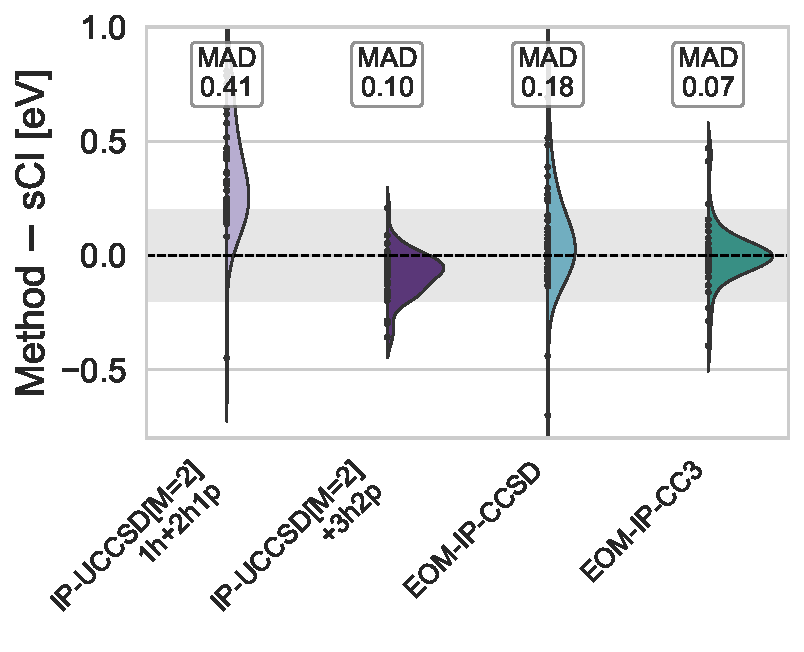
\includegraphics[width=\columnwidth]{figures/supinf_atz_violins}
\caption{Errors (method $-$ sCI, eV) of the IPs of the set of \citet{Marie_2024b}, aug-cc-pVTZ, frozen core, all 58 states.
IP-UCCSD[M=2]: UCCSD ground state with two nested commutators, cation space 1h+2h1p or with 3h2p added.
IP-EOM-CC values from Ref.~\citenum{Marie_2024b}.
Grey band: $\pm0.2$\,eV. Three 1h+2h1p errors and one IP-EOM-CCSD error lie above the plotted range.}
\label{fig:supinf_atz}
\end{figure}

Figure~\ref{fig:supinf_atz} shows the errors for the IPs of the set of \citet{Marie_2024b} in aug-cc-pVTZ with frozen core against the sCI reference.
The ground state is UCCSD with two nested commutators.
With the 1h and 2h1p configuration space, one recovers is the IP-qUCCSD method.
The IPs are too large, with a mean absolute deviation (MAD) of 0.41\,eV.
Adding the 3h2p configurations reduces the MAD to 0.10\,eV and the largest error from 1.52 to 0.36\,eV,
close to IP-EOM-CC3 (0.07\,eV, largest error 0.47\,eV).
The remaining error is a small, systematic underestimation, with a mean signed error of $-0.09$\,eV.




\appendix
\section{Generator input for UCCSD with 3h2p}
\label{app:complete}

The implementation passes the following operator expressions to the code generator, which expands them by Wick's theorem in spin orbitals.
The cluster operator is
\begin{equation}
\hs = \hat{T}_1 + \hat{T}_2 - \hat{T}_1^\dagger - \hat{T}_2^\dagger,
\label{eq:gen_sigma}
\end{equation}
with
\begin{equation}
\hat{T}_1 = \sum_{ia} t_i^a\, \hat{a}_a^\dagger \hat{a}_i, \qquad
\hat{T}_2 = \frac{1}{4}\sum_{ijab} t_{ij}^{ab}\, \hat{a}_a^\dagger \hat{a}_b^\dagger \hat{a}_j \hat{a}_i .
\label{eq:gen_T}
\end{equation}
The de-excitation amplitudes are entered as separate tensors and set equal to the excitation amplitudes at run time.
The Hamiltonian is the sum of the Fock operator and the fluctuation potential, both in normal order with respect to $\ket{\Phi_0}$, and both are transformed alike.
Every object below uses the same two-commutator Hamiltonian, Eq.~\eqref{eq:bch} with two commutators,
\begin{equation}
\Hb_2 = \hH + [\hH, \hs] + \frac{1}{2}[[\hH, \hs], \hs];
\label{eq:gen_hbar}
\end{equation}
no block is truncated at fewer commutators.

The ground-state energy and the amplitude equations are the projections
\begin{align}
E_0 &= \braket{\Phi_0 | \Hb_2 | \Phi_0}, \label{eq:gen_E0}\\
0 &= \braket{\Phi_0 | \hat{a}_i^\dagger \hat{a}_a\, \Hb_2 | \Phi_0}, \label{eq:gen_R1}\\
0 &= \braket{\Phi_0 | \hat{a}_i^\dagger \hat{a}_j^\dagger \hat{a}_b \hat{a}_a\, \Hb_2 | \Phi_0}, \label{eq:gen_R2}
\end{align}
which are solved iteratively with orbital-energy denominators and DIIS.

The cation operators of the three classes are those of Eq.~\eqref{eq:basis}, and the trial vector is
\begin{equation}
\hat{R} = \sum_i r_i\, \hat{a}_i + \frac{1}{2}\sum_{ija} r_{ij}^{a}\, \hat{a}_a^\dagger \hat{a}_j \hat{a}_i
+ \frac{1}{12}\sum_{ijkab} r_{ijk}^{ab}\, \hat{a}_a^\dagger \hat{a}_b^\dagger \hat{a}_k \hat{a}_j \hat{a}_i,
\label{eq:gen_R}
\end{equation}
with antisymmetric coefficients.
Each block of the matrix-vector product is generated separately as
\begin{equation}
\sigma_I^{(KL)} = \braket{\Phi_0 | \hat{q}_I^\dagger\, \Hb_2\, \hat{R}_L | \Phi_0},
\label{eq:gen_sigma_block}
\end{equation}
where $\hat{q}_I$ is a cation operator of class $K$ and $\hat{R}_L$ the class-$L$ part of Eq.~\eqref{eq:gen_R}, for all nine pairs of classes up to 3h2p.
The expansion is complete and contains disconnected terms.
Those that contain no external index sum to the ground-state energy times the trial vector, and the matrix of Eq.~\eqref{eq:M} is obtained by subtracting it,
\begin{equation}
\mathcal{M}\,\mathbf{r} = \boldsymbol{\sigma} - E_0\, \mathbf{r};
\label{eq:gen_M}
\end{equation}
those that contain the residuals of Eqs.~\eqref{eq:gen_R1} and \eqref{eq:gen_R2} vanish at convergence.

\bibliography{../../manuscript/biblio,extra}

\end{document}
